% Project:	Dashboard
% Title:	Dashboard: Track, analyze and decide 
% Description:	
% Author:	Héctor López


\documentclass[a4paper,12pt,english]{book}
% Comment the following to have chapters numbered without interruption (numbering through parts)
%\makeatletter\@addtoreset{chapter}{part}\makeatother%

%
% Required packages
%
\usepackage[english]{babel}		% language
\usepackage[utf8]{inputenc}		% para acentos y eñes
\usepackage{graphicx}			% graphics in jpeg, png or pdf format
\usepackage{titleref}
\usepackage{tocbibind}
\usepackage{hyperref}			% generates PDF links
\usepackage{multicol}			% for multicolumns
\usepackage{subfigure}
\usepackage{multirow}
\usepackage{listings}			%Sourcecode
\usepackage[toc,page]{appendix}
\usepackage{color}
\usepackage{framed}

\definecolor{codegreen}{rgb}{0,0.6,0}
\definecolor{codegray}{rgb}{0.5,0.5,0.5}
\definecolor{codepurple}{rgb}{0.58,0,0.82}
\definecolor{backcolour}{rgb}{0.95,0.95,0.92}
\definecolor{gray97}{gray}{.97}
\definecolor{gray75}{gray}{.75}
\definecolor{gray45}{gray}{.45}


\lstdefinestyle{html}{
	language=html,
    frame=Ltb,
	framerule=0pt,
	aboveskip=0.5cm,
	framextopmargin=3pt,
	framexbottommargin=3pt,
	framexleftmargin=0.4cm,
	framesep=0pt,
	rulesep=.4pt,
	numbers=left,
	numbersep=15pt,
	numberstyle=\tiny,
	numberfirstline = false,
	breaklines=true,
	rulesepcolor=\color{black},
    backgroundcolor=\color{backcolour},   
    commentstyle=\color{codegreen},
    keywordstyle=\color{magenta},
    numberstyle=\tiny\color{codegray},
    stringstyle=\color{codepurple},
    %basicstyle=\small\sffamily,
    basicstyle=\scriptsize,
    breakatwhitespace=false,         
    captionpos=b,                    
%     keepspaces=true,                 
%     showspaces=false,                
%     showstringspaces=false,
%     showtabs=false,                  
%     tabsize=2
}

\lstdefinestyle{sql}
{
	language=sql,
    frame=Ltb,
	framerule=0pt,
	aboveskip=0.5cm,
	framextopmargin=3pt,
	framexbottommargin=3pt,
	framexleftmargin=0.4cm,
	framesep=0pt,
	rulesep=.4pt,
	numbers=left,
	numbersep=15pt,
	numberstyle=\tiny,
	numberfirstline = false,
	breaklines=true,
	rulesepcolor=\color{black},
    backgroundcolor=\color{backcolour},   
    commentstyle=\color{codegreen},
    keywordstyle=\color{magenta},
    numberstyle=\tiny\color{codegray},
    stringstyle=\color{codepurple},
    %basicstyle=\small\sffamily,
    basicstyle=\scriptsize,
    breakatwhitespace=false,         
    captionpos=b,                    
%     keepspaces=true,                 
%     showspaces=false,                
%     showstringspaces=false,
%     showtabs=false,                  
%     tabsize=2
}

% minimizar fragmentado de listados
\lstnewenvironment{listing}[1][]
{\lstset{#1}\pagebreak[0]}{\pagebreak[0]}

\lstdefinestyle{console}
{
	language=shell,
	basicstyle=\scriptsize\bf\ttfamily,
	backgroundcolor=\color{gray75},
	commentstyle=\color{codegreen},
    keywordstyle=\color{magenta},
    numberstyle=\tiny\color{codegray},
    stringstyle=\color{codepurple},
}

\lstdefinestyle{c}
{
	language=html,
	frame=Ltb,
	framerule=0pt,
	aboveskip=0.5cm,
	framextopmargin=3pt,
	framexbottommargin=3pt,
	framexleftmargin=0.4cm,
	framesep=0pt,
	rulesep=.4pt,
	backgroundcolor=\color{gray97},
	rulesepcolor=\color{black},
	%
	stringstyle=\ttfamily,
	showstringspaces = false,
	basicstyle=\small\ttfamily,
	commentstyle=\color{gray45},
	keywordstyle=\bfseries,
	%
	numbers=left,
	numbersep=15pt,
	numberstyle=\tiny,
	numberfirstline = false,
	breaklines=true
}

\lstdefinelanguage{JavaScript}{
  morekeywords={typeof, new, true, false, catch, function, return, null, catch, switch, var, if, in, while, do, else, case, break},
  morecomment=[s]{/*}{*/},
  morecomment=[l]//,
  morestring=[b]",
  morestring=[b]'
}

\lstset{style=html}

\renewcommand{\theTitleReference}[2]{\chaptername{}\ #1:\ \emph{#2}}
\newcommand{\reffigure}[1]{\figurename{}\ \ref{#1}} 

%
% Page set up
%
%\oddsidemargin -1.0cm
%\headsep -2.4cm
%\textwidth=18.5cm
%\textheight=26cm

\newenvironment{dedication}
{
   \cleardoublepage
   \thispagestyle{empty}
   \vspace*{\stretch{1}}
   \hfill\begin{minipage}[t]{0.15\textwidth}
   \raggedright
}%
{
   \end{minipage}
   \vspace*{\stretch{3}}
   \clearpage
}

%
% PFC 
%
\begin{document}
\clearpage\thispagestyle{empty}
\vspace*{\fill}
\begin{framed}
	\begin{center}
	Universitat de Lleida \\ \medskip
	Escola Politècnica Superior \\ \medskip
	Enginyeria en Informàtica \\ \bigskip \bigskip
	
	Sistemes informàtics (Treball de final de carrera) \\ \bigskip \bigskip 
	
	\textbf{Dashboard: Track, analyze and decide}
	\end{center}

	\bigskip
	
	\raggedleft
	Autor: Héctor López Sacanell\\
	Directors: Juan Manuel Gimeno i Roberto García\\
	Setembre de 2014
	\bigskip
\end{framed}
\vfill
\clearpage

\title{Dashboard: Track, analyze and decide}
\author{Héctor López}
\inputencoding{utf8}

\date{\today}
%\maketitle

\begin{dedication}
A Silvia :)
\end{dedication}

%\input{portada.tex}

\tableofcontents

% Agradecimientos
\newpage
\thispagestyle{empty}
 \chapter*{Acknowledgments}
 \addcontentsline{toc}{chapter}{Acknowledgments}
First of all I would like to thank Silvia for the constant support and effort
she gave me to carry out this project.\\

I would also like to thank Juan Manuel and Roberto for the long
and constant support they gave me till the last moment. Something I really
appreciate and I am sure it is appreciated by their colleagues as well. \\

Last but not the least, I would really thank the open source community and the
constant work and initiatives that the online world that has boosting every day
new ways to do things and raise improvements for the 3rd needs. Without all this
people, this project could not be possible.
 

\chapter*{Source Code}
\addcontentsline{toc}{chapter}{Source Code}
All code has been pushed to \url{https://github.com/beldog/dashboard}
repository, as well this document under \url{https://github.com/beldog/dashboard-doc} repository.

\chapter*{Motivation}
\addcontentsline{toc}{chapter}{Motivation}
In order to track and follow up project's status, my colleagues and I
built, on 2013, a simple tool in a spreadsheet that linked with a database that
allowed us to log each change (aka \emph{event}) on the project status of on
the following scope: phase change end/start, delay, launch.

This tool also gave us a good view about different selected KPI \footnote{Key
Performance Indicator}. And based on those indicators some reports can be
built:
Project's events, Project's launched, Project's delayed (and detail), Project's
Gantt and Project's timelines.

The tool was fine for a while, but it took too much time to load all data
from the database, and also was not fully accessible for all users, because
of the need to install some extra required components like the ODBC for those with
Windows, or not even compatible with those using Linux computers, because the
tool was built on Microsoft Excel.

So, imagine trying to track project's \emph{events} on a tool that is slow
and not compatible with everybody. At the end we stopped using it.

Then, a fresh motivation came up to build something better,
usable for all required users and faster enough to aim the objective: track,
analyze and decide. 

The challenge was both there and as well the information on the database, so it
was just a matter to migrate the spreadsheet (the view) to a HTML page with some JS,
as first client, so we decouple it from any need of 3rd party component such as
ODBC, having in the middle a RESTful service that
controls the communication between the client (web browser) and what matters,
the data (our business).

\chapter*{Planning}
\addcontentsline{toc}{chapter}{Planning}
Now that you know what is the main objective, next step is to break it down in
small parts and assign timelines.

Three different phases has been defined:
\begin{itemize}
	\item Phase 1: Migrate current spreadsheet dashboard to simple REST +
	HTML/JS
	\item Phase 2: Implement Dashboard view with HTLM5/CSS3/JS
	\item Phase 3: Automate dependencies linking Dashboard with 3rd ticketing
	tool
\end{itemize}

Moreover, this project was forecasted as 6 month project but extended on
the time to 9 months, because the time expected to be invested per day is less
than half working day top. So forecasted timelines were defined as follows:

\begin{figure}[ht!]
	\centering
   	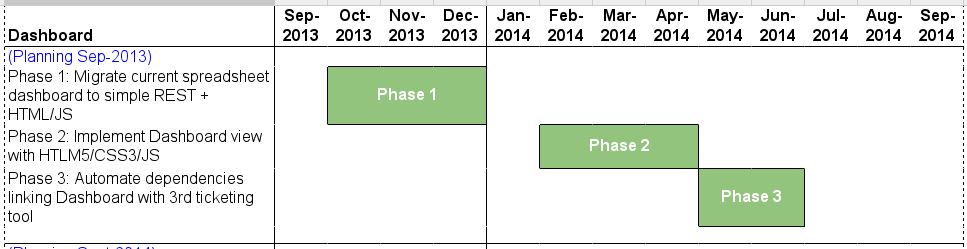
\includegraphics[width=1\textwidth]{./resources/planning_baseline_12pt.png}
   	\caption{Planning Baseline}
   	\label{f_planning_baseline}
\end{figure}

Main process followed has been the \emph{Lean approach}, where we have
dedicated part of the time to get documented on new frameworks or APIs
that we could use in order to don't reinvent the wheel, and as soon as we
learned about the new technology, then we build a small piece of the final tool,
so we can see and check out how it performs and increase the complexity or
correct the issues later on, but with a working piece of the tool.

But life has always time for surprises and good presents, and mentioned
timelines were badly impacted because of two main reasons: \emph{I became a father} and
\emph{I was promoted at work}. Be a father is one of the most wonderful things
I have ever lived, but has its own downsides, like any plan that you
built before the birth gets automatically outdated. And this is what happened
with the plan shown above. So we ended with the following timelines: 

\begin{figure}[ht!]
	\centering
   	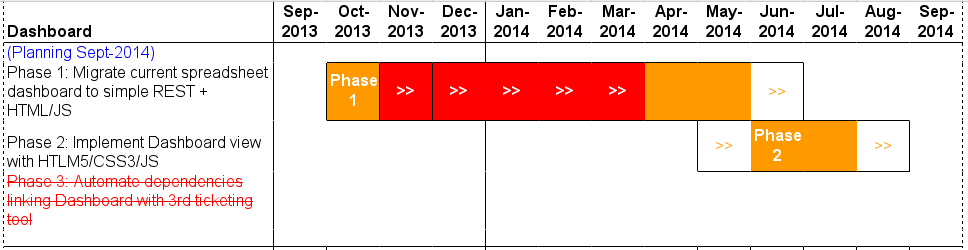
\includegraphics[width=1\textwidth]{./resources/planning_sep2014_12pt.png}
   	\caption{Final Timelines}
   	\label{f_planning_final}
\end{figure}

As you can see, Phase 1 has been delayed for almost 5 months. Of course those 5
months has not been 0\% investment, but the productivity on this period was
around 5\%.

Once Phase 1 was fineshed (middle June\/2014), a replanning was required, and
the output was to cancelled Phase 3 and leave it as future work.

%
% Chapters
%
\part{Migrate Excel spreadsheet dashboard to a simple REST+HTML/JS
application}
\label{c_phaseone}

\chapter*{Motivation}
\addcontentsline{toc}{chapter}{Motivation}
In order to track and follow up project's status, we built a simple tool in a
spreadsheet that linked with a database allowed us to log each change (aka
\emph{event}) on the project status on the following scope: phase change
end/start, delay, launch.

This tool also gave us a good view about different selected KPI \footnote{Key
Performance Indicator}. And based on those indicators we built few reports:
Project's events, Projects launched, Projects delayed (and detail), Projects
Gantt and Project's timelines.

The tool was fine for a while, but it took to much time to load all data
from the database, and also was not fully compatible with all users, because of
the need to install some extra required components like the ODBC for those with
Windows, or not even compatible with those using Linux computers, because the
tool was built on Microsoft Excel.

So, imagine trying to track project's \emph{events} on a tool that is slow
and not compatible with everybody. At the end we stopped using it.

Then, a fresh motivation came up to build something better,
usable for all required users and faster enough to aim the objective: track,
analyze and decide. 

The challenge was there and as well the information on the database, so it was
just a matter to migrate the spreadsheet (the view) to a HTML page with some JS,
as first client, so we decople it from any need of 3rd party component such as
ODBC, having in the middle a RESTful service that
controls the communication between the client (web browser) and what matters, the data (the model).

\chapter{Current Excel architecture}
At the beginning, the idea was to have the data centralized
\label{t_main_objective} and implement, in a fast way, a client that could show
it. The quicker solution, not always the right one but useful for a while, was
to define the simpliest database model to  track the maximum amount of events with enough value to evaluate a the
efficiency of a project and learn from our mistakes. Together with the database
we setup a Excel spreadsheet that loads the data from the defined database, but
we also needed to build different reports, so we difined few \emph{views} based
on the required KPIs, so we could query it from the external spreadsheet
without define any kind of logic, that could increase the complexity.\\

In short, elements defined are listed as follow:
\begin{itemize}
  \item A MySQL database with one table called Events used to store any possible
  event (previously defined the set of them)
  \item Few views used to achieve defined reports
  \item A Microsoft Excel spreadsheet used to show data returned by the views
  \item One connection per report used to connect Excel with the database
  via ODBC as data connectivity abstractor. 
\end{itemize}

You can see the relationship between above listed components on the 
\reffigure{f_excel_architecture}.
 
\begin{figure}[ht!]
	\centering
   	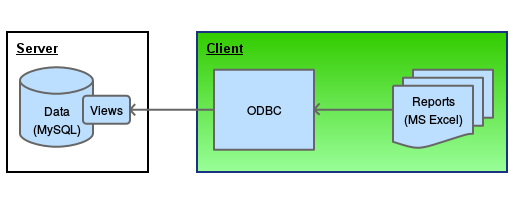
\includegraphics[width=1\textwidth]{./resources/excel_architecture.png}
   	\caption{Reports architecture using Excel}
   	\label{f_excel_architecture}
\end{figure}

\section{Database model}
Database model was defined as simple as possible, keeping in mind
possible normalization in the future without having a big impact on the data. So
decission was to use
\emph{Enum}\footnote{https://dev.mysql.com/doc/refman/5.0/en/enum.html} data
type for those fields that are static or with a predefined set of
elements like: country, project\_type or  type fields
(\reffigure{f_data_model}).

\begin{figure}[ht!]
	\centering
   	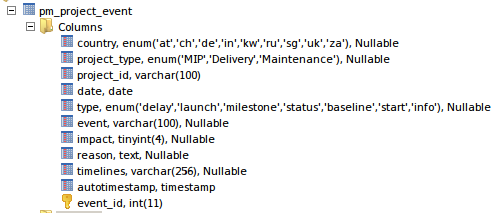
\includegraphics[width=1\textwidth]{./resources/data_model.png}
   	\caption{Data model}
   	\label{f_data_model}
\end{figure}

The most relevant field here is \emph{type}, where covers all required possible
scenarios in a project's lifetime that we needed to track. And base on that, 
reports (views) can show the specific information to be analyzed.

\section{Views definition and reports}
As described on the previous sections, we defined five reports, they are:

\begin{itemize}
  \item Amount of launches, per country and month
  \item Total project's delay
  \item Project's delays in detail
  \item Gantt chart
  \item Project's timelines chart 
\end{itemize}

On top of them, we also added an extra report listing all project's events,
just for our reference.

You can see screenshots on how they look for each of them on
\reffigure{f_report_launches}, \reffigure{f_report_delays},
\reffigure{f_report_delays_detail}, \reffigure{f_report_gantt},
\reffigure{f_report_timelines} and \reffigure{f_report_events}.

\begin{figure}[ht!]
	\centering
   	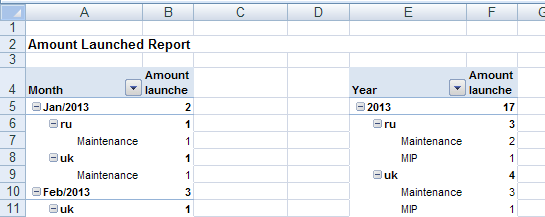
\includegraphics[width=1\textwidth]{./resources/report_launches.png}
   	\caption{Launches report}
   	\label{f_report_launches}
\end{figure}
\begin{figure}[ht!]
	\centering
   	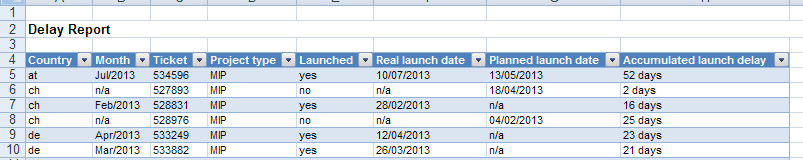
\includegraphics[width=1\textwidth]{./resources/report_delays.png}
   	\caption{Delays report}
   	\label{f_report_delays}
\end{figure}
\begin{figure}[ht!]
	\centering
   	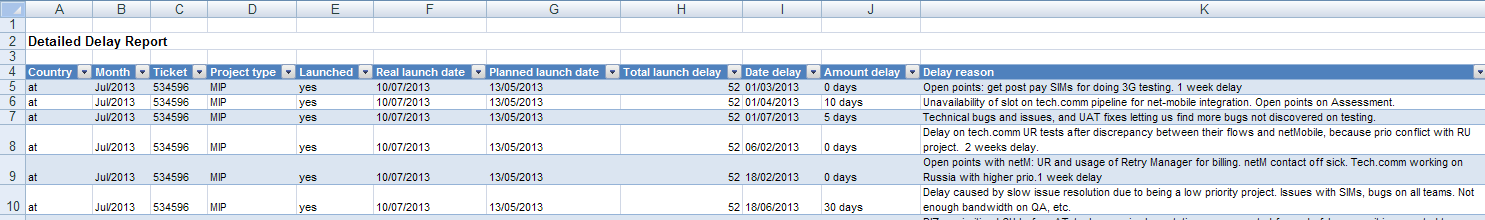
\includegraphics[width=1\textwidth]{./resources/report_delays_detail.png}
   	\caption{Detailed delays report}
   	\label{f_report_delays_detail}
\end{figure}
\begin{figure}[ht!]
	\centering
   	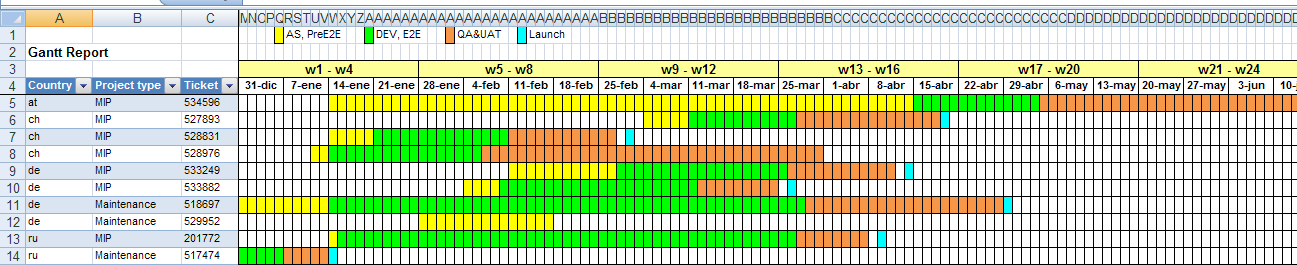
\includegraphics[width=1\textwidth]{./resources/report_gantt.png}
   	\caption{Gantt report}
   	\label{f_report_gantt}
\end{figure}
\begin{figure}[ht!]
	\centering
   	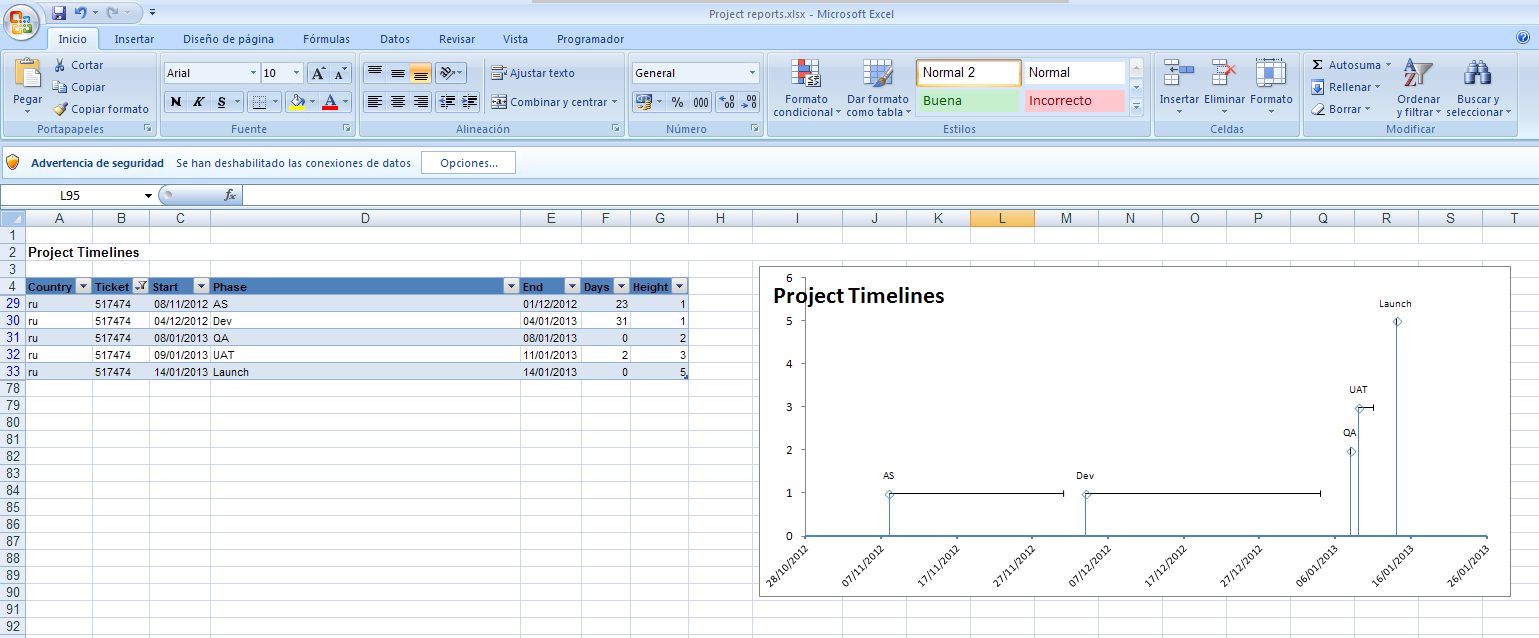
\includegraphics[width=1\textwidth]{./resources/report_timelines.png}
   	\caption{Timelines report}
   	\label{f_report_timelines}
\end{figure}
\begin{figure}[ht!]
	\centering
   	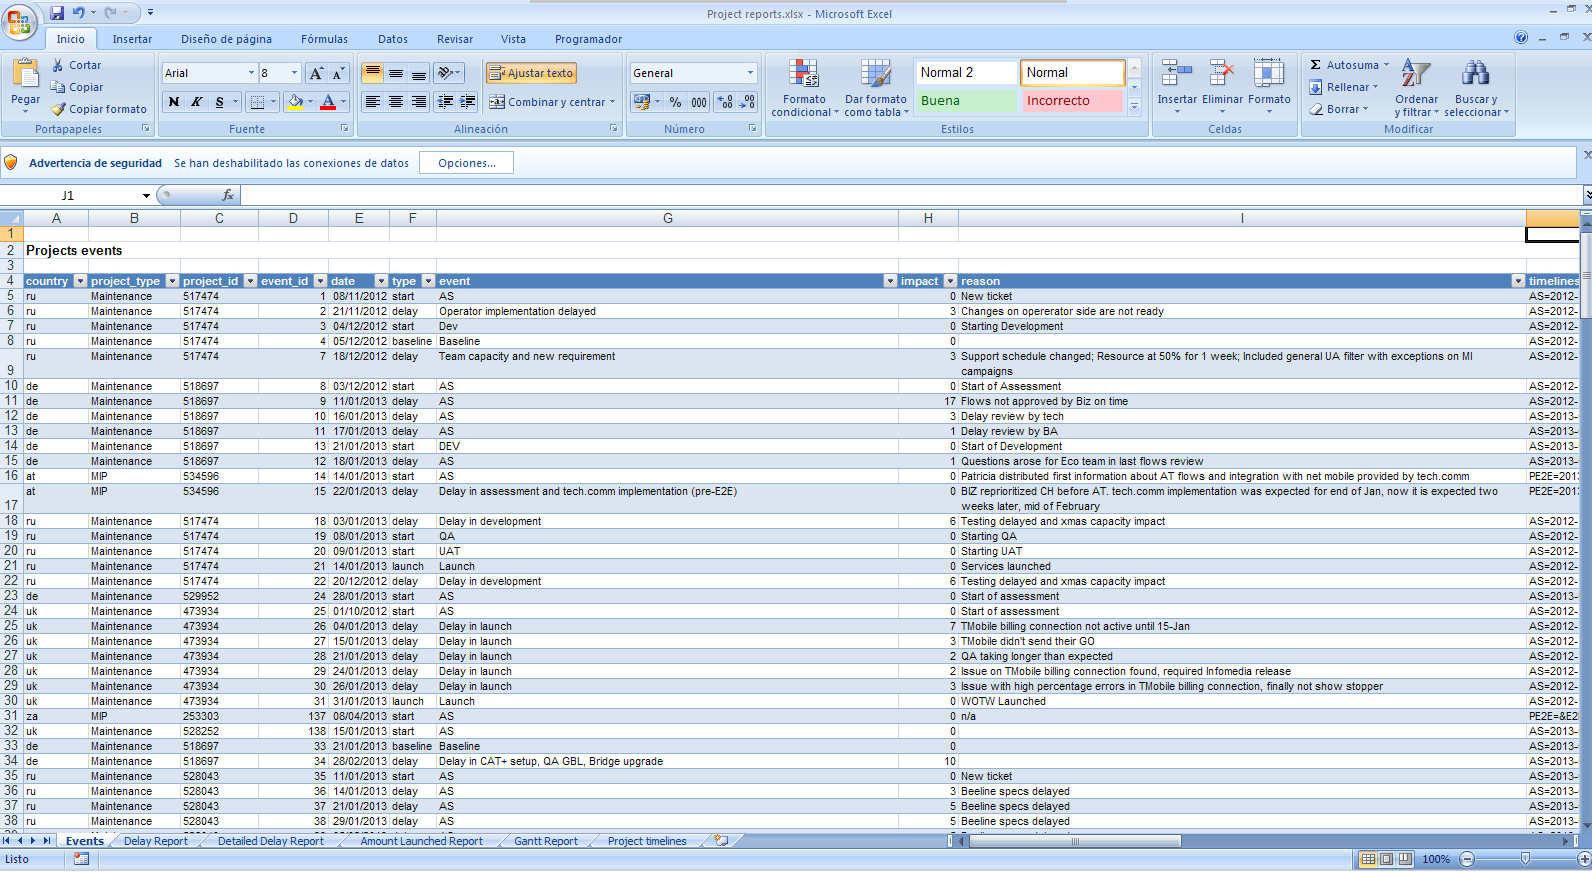
\includegraphics[width=1\textwidth]{./resources/report_events.png}
   	\caption{Events report}
   	\label{f_report_events}
\end{figure}

Each of those reports has defined one or more than one table's view that execute
the required data calculations and format the output in a Excel friendly way, so
the spreadsheet just need to show it and doesn't require any customization. 

This data and format coupling on the views definition was done on purpose,
in order to be flexible enough in the future in case was needed to define a
different viewer component, a part of the Excel, such as and HTML, or just
migrate it to a different platform. But, on both case the model could remain
untouched if the objective remained the same and only is needed to change the
view with a more powerful or friendly one. See and example on
\ref{f_report_launchesbymonth}.

\lstinputlisting[language=SQL,breaklines=true,caption=Launches
by month
view,label=f_report_launchesbymonth,frame=single,captionpos=b]{resources/report_launchesbymonth.sql}

In the other hand, decoupling it will need to be taken sooner or later if
we want to have a flexible and scalable tool, but this will be part of the
future work.

\section{The issue and what to improve}
As slightly tackle on previous sections, building a reporting tool based on
Excel was not the better solution, but it covered the main needs, even if we
faced issues like slowness, a single shared spreadsheet to be used by all
project managers, every report has a standalone database connection with the
possible impact on resources it could have and manual database insert per
each project's event.

All these points will be reviewed and covered on the next chapter. 

\chapter{New RESTful architecture}
After few time working with the spreadsheet linked with the database, and having
listed its downsides, I have started thinking about how to improve it without
affecting the main objective \ref{t_main_objective} but making it more
user friendly.

We already had listed the weaknesses and thinking on one by one, just came up
that the main change would be to replace completly the view (Excel), that
will solve all the issues, but will lose the power of the pivot table and
filters, but it could be managed in a second or third stage.

Now the question is: what could be the best replacement?

\section{Looking for a view replacement}


\chapter{Migration plan}

\chapter{Conclusions}

\chapter{Future work}
\begin{itemize}
	\item Refactor database connectivity using a proper JPA based framework.
  
	Implement a real database connection pool using one of the existing persistence
	frameworks that implements JPA\footnote{Java Persistence API:
	\url{http://www.oracle.com/technetwork/articles/javaee/jpa-137156.html}}.
	
	\item Remove data-format coupling returned to the client.
	\item Refactor client making it usable for the final user (requires assessment
	and evaluation of main actions to carry out by the user).
\end{itemize}

%\begin{appendices}
%\chapter{Table views reports}
%\lstinputlisting[language=SQL,breaklines=true]{resources/reports_views.sql}
%\end{appendices}

\part{Phase Two: Implement Dashboard view with HTLM5/CSS3/JS + extend RESTful
API}

\chapter*{Introduction}
\label{c_phasetwo}
On this section, we will experiment with different frameworks to improve the
tool in terms of UX and functionality. Also we will look for new ways to show
same data, just following a Lean approach and go step by step until the result
is the successful one.


\chapter{Facelift with Bootstrap}
There are few front end frameworks that help the web developer to build a
consistent, usable and responsive web, such as
Backbone\footnote{\url{http://backbonejs.or}}, 
Underscore\footnote{\url{http://underscorejs.org/}},
Skeleton\footnote{\url{http://www.getskeleton.com/}},
Foundation\footnote{\url{http://foundation.zurb.com/}},
Compass\footnote{\url{http://compass-style.org/}},
Bootstrap\footnote{\url{http://getbootstrap.com/}} and few others. With them
you cover the required features to build a web tool in a
single page and/or have responsive mobile web implementation using the latest
CSS3 and Saas extension, like Compass.

I started applying Bootstrap to the dashboard in a very straight forward way and
getting awesome results a couple of hours later.

First thing to do is to import required libraries, such as main style sheet,
JavaScript extensions (that is required to get some fancy actions and effects)
and optional theme, as it is shown on the following code
\ref{f_facelift_bootstrap_code}, note that the library is loaded from the
closest server to the user as it is using \emph{MaxCDN.com} service
(\texttt{//maxcdn.bootstrapcdn.com/\ldots}), being a distributed replication
content system\footnote{Other similar system would be
\url{http://www.akamai.com}.}.

\begin{lstlisting}[style=html,breaklines=true,caption=Bootstrap\
required\ libraries,label=f_facelift_bootstrap_code]
<!-- Bootstrap http://getbootstrap.com/getting-started/ --> 
<!-- Latest compiled and minified CSS --> 
<link rel="stylesheet" href="//maxcdn.bootstrapcdn.com/bootstrap/3.2.0/css/bootstrap.min.css">

<!-- Optional theme -->
<link rel="stylesheet" href="//maxcdn.bootstrapcdn.com/bootstrap/3.2.0/css/bootstrap-theme.min.css">

<!-- Latest compiled and minified JavaScript -->
<script src="//maxcdn.bootstrapcdn.com/bootstrap/3.2.0/js/bootstrap.min.js"></script>
<!-- Bootstrap -->
\end{lstlisting} 

Once we have the style sheet loaded, we just need to apply to our html entities
the proper class and role and result is just so fancy as you can see on the
following \reffigure{f_facelift_bootstrap},
\reffigure{f_facelift_bootstrap_2} and \reffigure{f_facelift_bootstrap_3}.

\begin{figure}[ht!]
	\centering
   	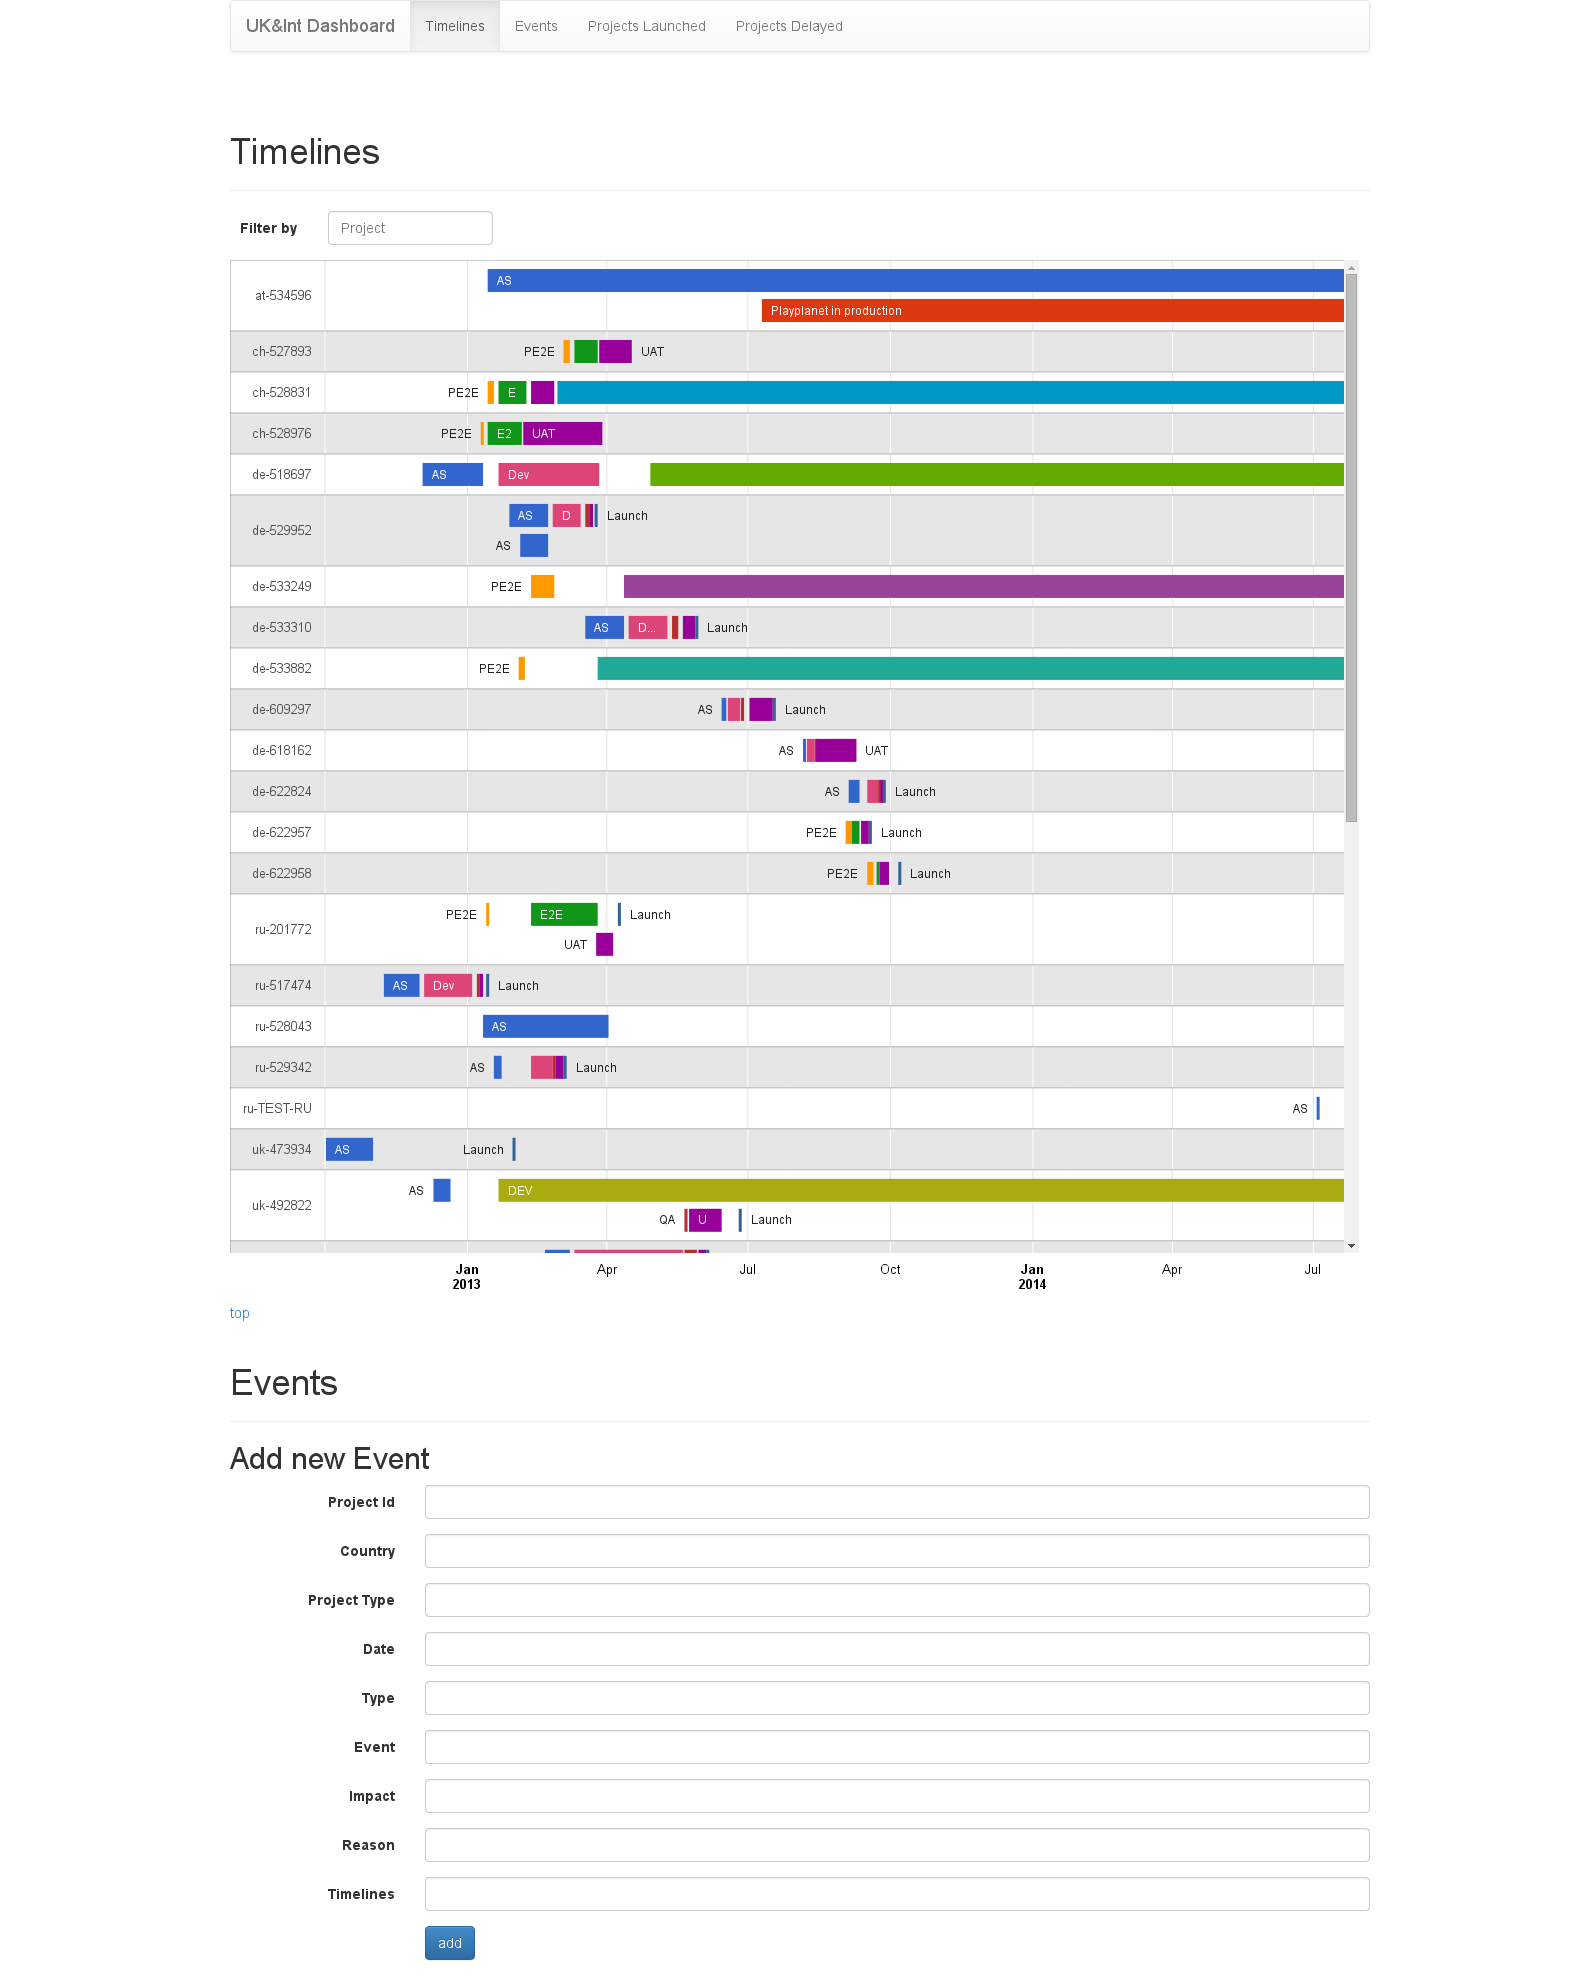
\includegraphics[width=1\textwidth]{./resources/dashboard_after_bootstrap_1.png}
   	\caption{Dasboard look and feel after apply Bootstrap style sheet (1)}
   	\label{f_facelift_bootstrap}
\end{figure}

\begin{figure}[ht!]
	\centering
   	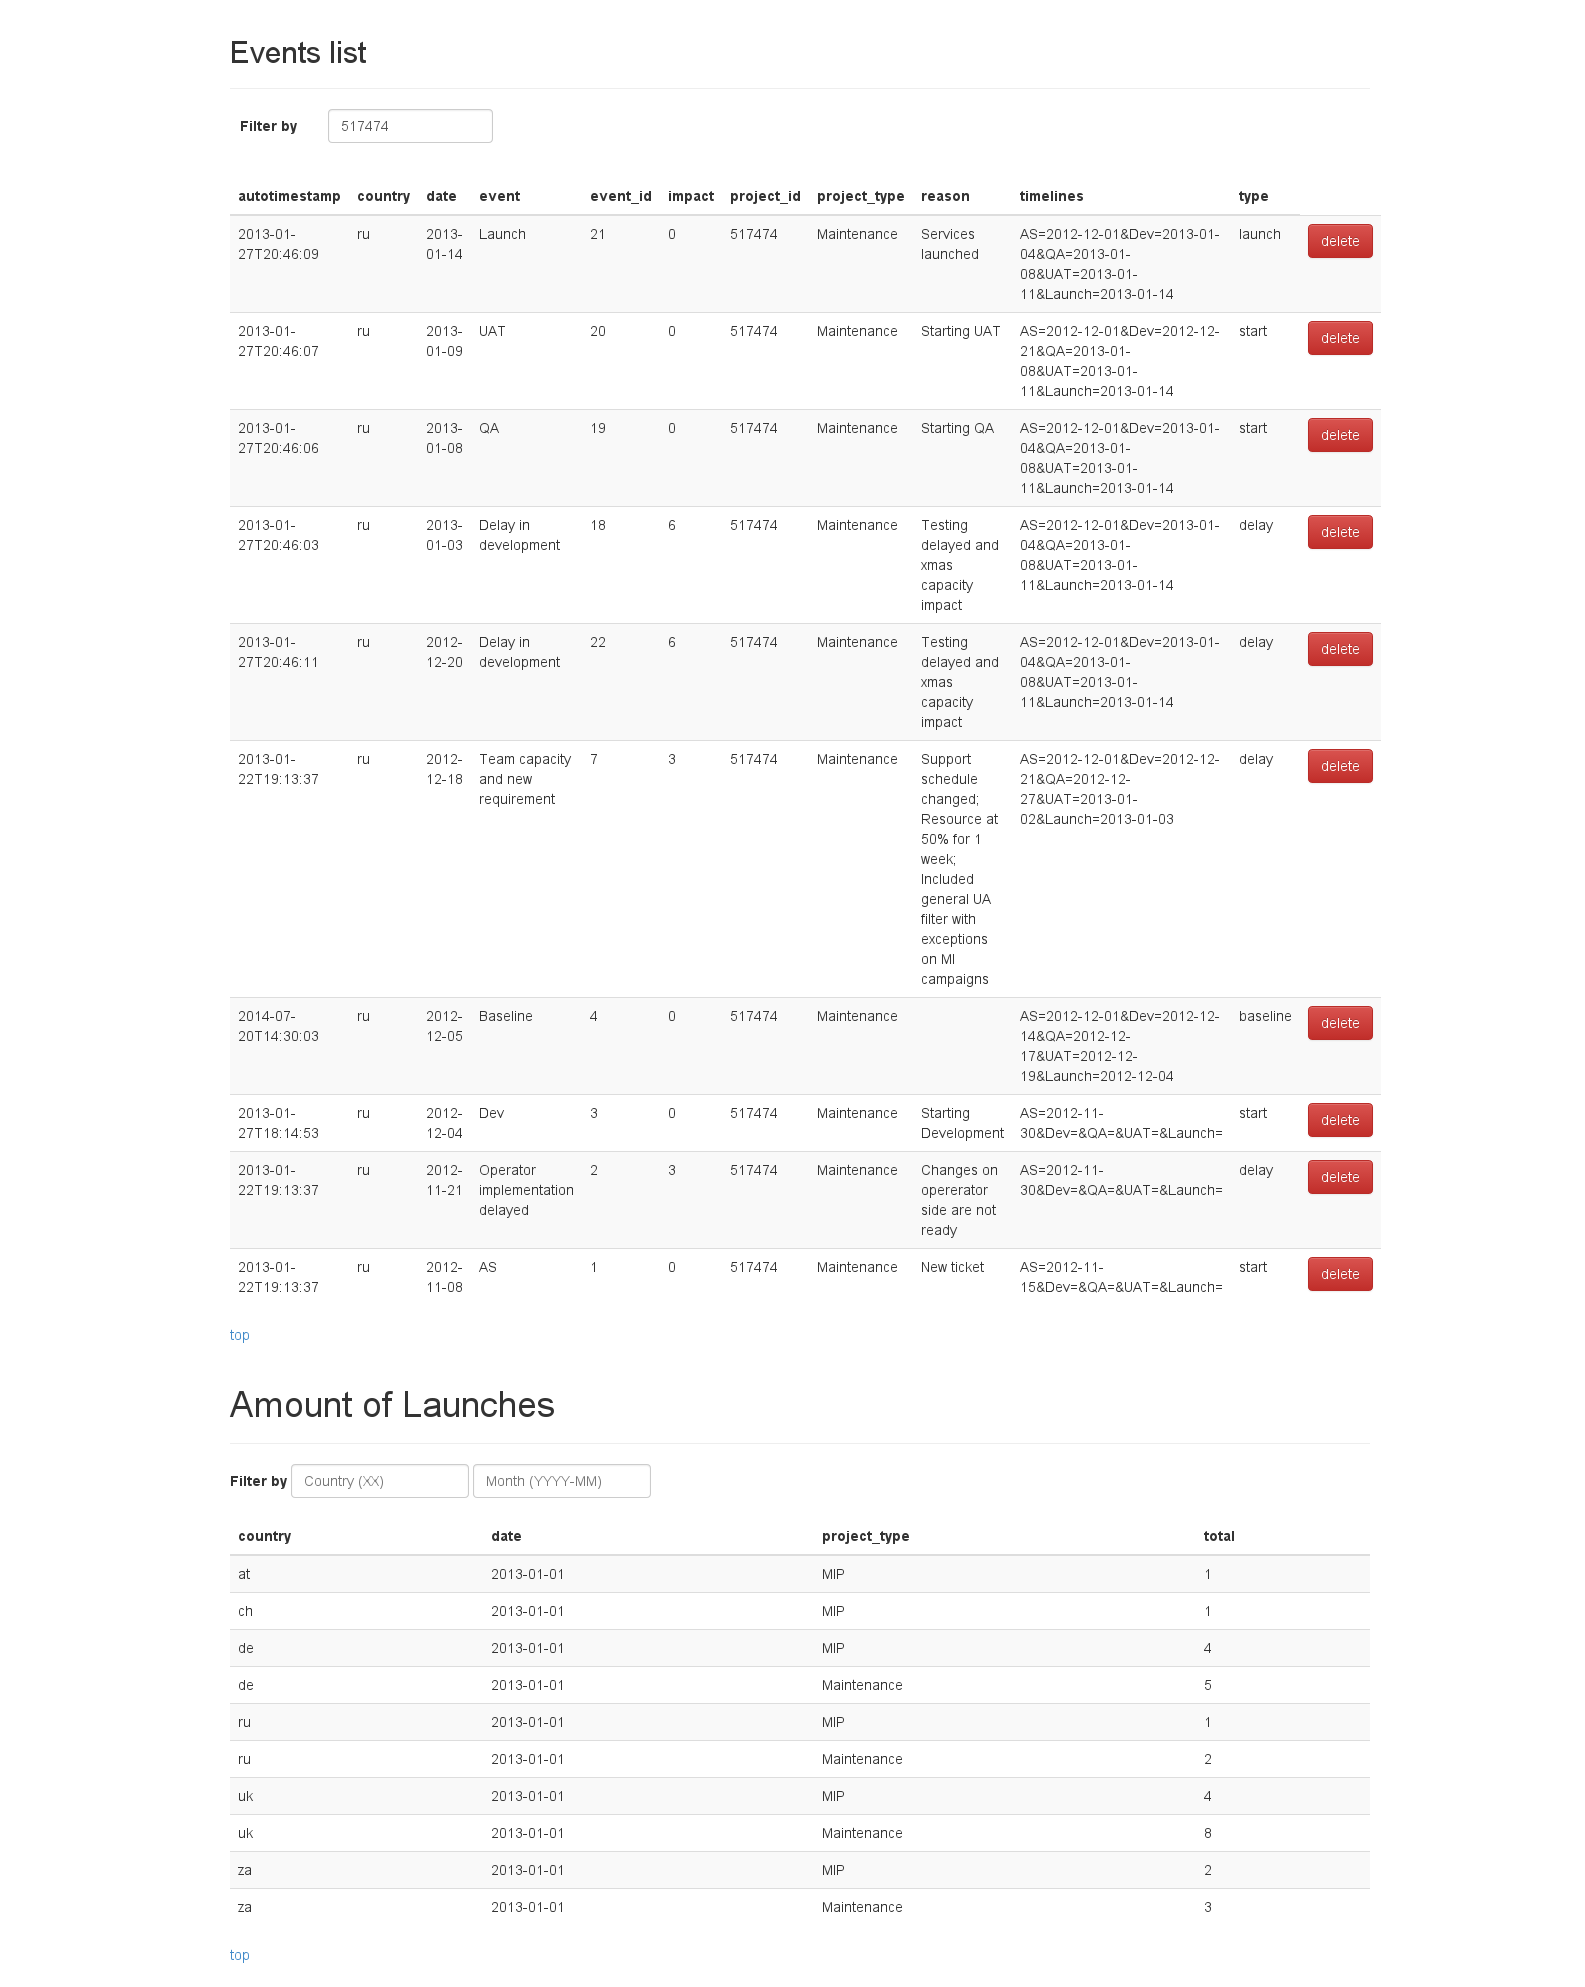
\includegraphics[width=1\textwidth]{./resources/dashboard_after_bootstrap_2.png}
   	\caption{Dasboard look and feel after apply Bootstrap style sheet (2)}
   	\label{f_facelift_bootstrap_2}
\end{figure}

\begin{figure}[ht!]
	\centering
   	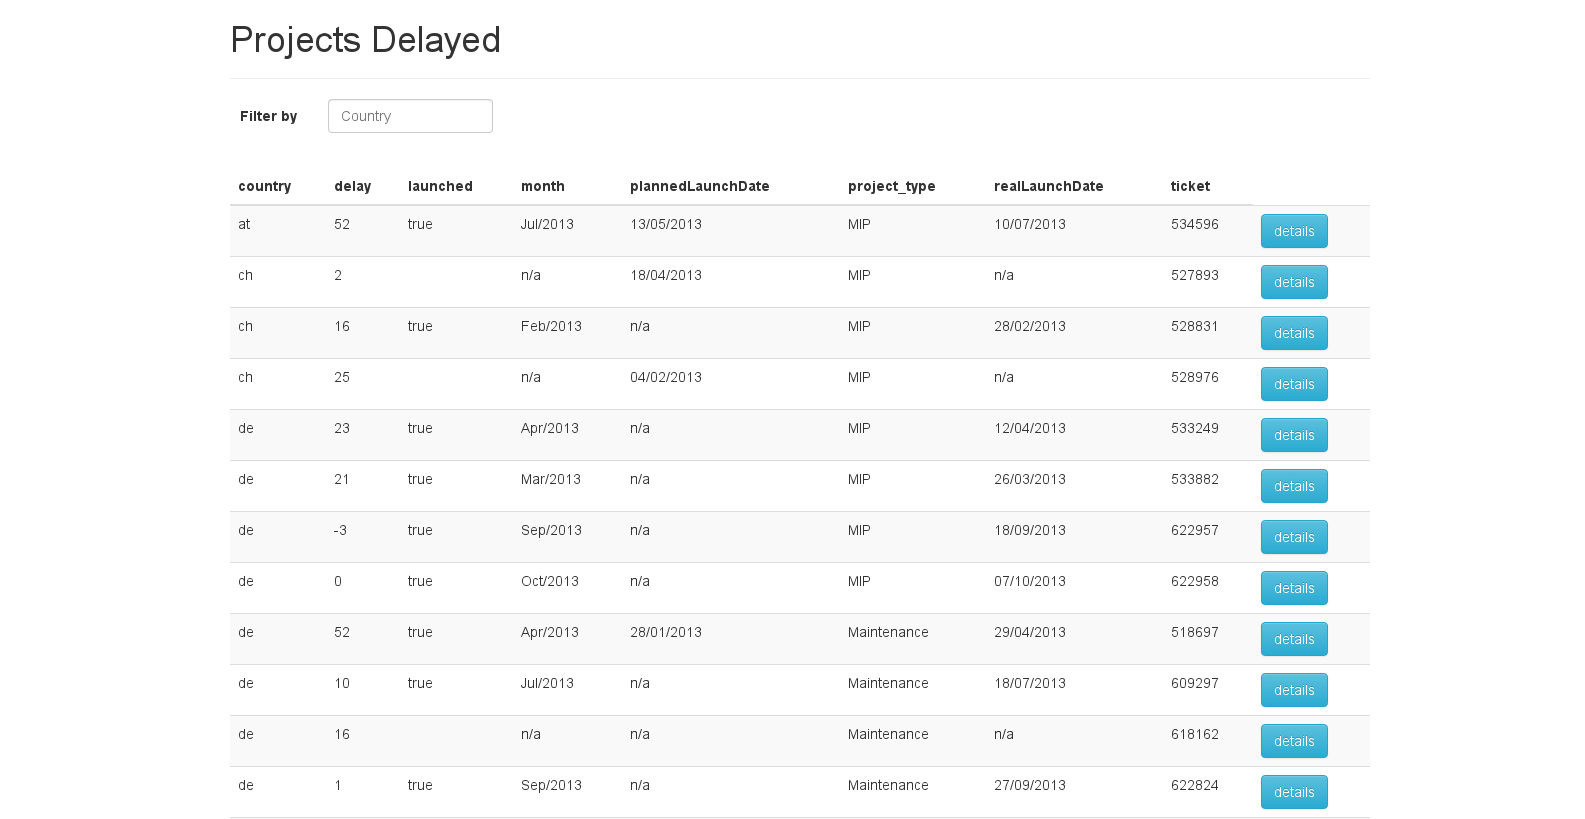
\includegraphics[width=1\textwidth]{./resources/dashboard_after_bootstrap_3.png}
   	\caption{Dasboard look and feel after apply Bootstrap style sheet (3)}
   	\label{f_facelift_bootstrap_3}
\end{figure}

\chapter{Extending Dashboard with Elasticsearch and Kibana}
Working on this currently and see if is feasible to implement the searching and
data calculation required for the reports based on Elasticsearch. The
main interesting point here is that we can change the way that we have been
thinking about the data on this project, and switch it from a relational data
model (MySQL), to a noSQL approach using Document model (JSON), something that our
application already uses :)

Don't know where it will end, but let's see and have fun with it along the
process.


\begin{part}{Conclusions and Future work}

%\chapter{Introduction}
%\label{c_phasethree}


\chapter{Conclusions}
There is a wide variety of ways to do the same thing, also frameworks and
technologies to use. The ones used until now on this project are just an example
of the technologies that fits the project needs but it doesn't mean they are the best
ones, but at least covers the main objective being compliance with it in a
short-mid term. But, as technology changes every day, the most important part is
to isolate (or decouple) your main business logic out of the technology used.
So, if in the future you are force to change the ecosystem, at least you can ensure your
logic will not change drastically and you can migrate it from one system to
another.\\

Building a tool usually requires significant time for coding what you have
defined on the Use/Business cases, but a major part of the time is also used to
assess and evaluate which tools/frameworks provide the open source community
that could be reused and fit on your own project. This investment on reusing
components from 3rd is a common practise and it will safe value time that you
could invest on other tasks. 
In the same way that reusing Bootstrap or Google
Charts provides a good result without any need to invest time on coding it from
scratch rather than read the API.\\

All in all, the tool that has been built on this time still has room for
improvements, but it is already in a stage where it can be used on a daily basis
to track daily project's events and in parallel keep working on extend it and
provide new features that will help the Project managers to track, analyze and
decide next actions for their projects.

\chapter{Future work}
We left out of this part improvements and things to do better, but they will be
covered on future work, such as:


\begin{itemize}
	\item Refactor database connectivity using a proper JPA based
	framework\footnote{Java Persistence API:
	\url{http://www.oracle.com/technetwork/articles/javaee/jpa-137156.html}}.
	\item Remove data-format coupling returned to the client.
	\item Refactor client making it usable for the final user (requires assessment
	and evaluation of main actions to carry out by the user and role).
	\item Refactor client code architecture using Backbone.js and Underscore.js
	\item Implement rest of listeners and actions required on CHAP Links Timeline
	chart to build a full interactive chart.
	\item Automate dependencies linking projects with 3rd ticketing tools.
	\item Define and implement a performance and evaluation system able to detect
	risk, and calculate&evaluate main KPIs.
\end{itemize}
\end{part}


\cleardoublepage
\phantomsection
\addcontentsline{toc}{part}{Bibliography}
\begin{thebibliography}{1}

	\bibitem{}{}{\em ``Jersey 2.10.1 User Guide''}. \url{https://jersey.java.net}.
	\bibitem{}{} 
		{\em ``Understanding JDBC internals and timeouts configuration''}.
		\url{http://www.cubrid.org/blog/dev-platform/understanding-jdbc-internals-and-timeout-configuration/}.
	\bibitem{}{}{\em ``Stackoverflow web site''}. \url{http://stackoverflow.com/}.
	\bibitem{}{}{\em ``Google Charts documentation''}.
	\url{https://google-developers.appspot.com/chart/interactive/docs/gallery}.
	\bibitem{}{}{\em ``Microsoft Excel Overview of connectiong to import data''}
	\url{http://office.microsoft.com/en-us/excel-help/overview-of-connecting-to-importing-data-HP010342748.aspx}.
	\bibitem {}{}{\em ``Bootstrap user guide''}. \url{http://getbootstrap.com/css/}
	and \url{http://getbootstrap.com/components/}.
	\bibitem{}{}{\em ``CHAP Links Timelines
	API}{\url{http://almende.github.io/chap-links-library/js/timeline/doc/}} 
% 	\bibitem{}{}{\em ``Elasticsearch Guide''}.	\url{http://www.elasticsearch.org/guide/}.
% 	\bibitem{}{Clinton Gormley}{\em ``Getting down and dirty with Elasticsearch''}.
% 	\url{https://www.youtube.com/watch?v=52G5ZzE0XpY}
% 	\bibitem{}{Frank Evers}{\em ``Four ways to index relational data in
% 	Elasticsearch''}.
% 	\url{http://voormedia.com/blog/2014/06/four-ways-to-index-relational-data-in-elasticsearch}.
\end{thebibliography}

\end{document}